		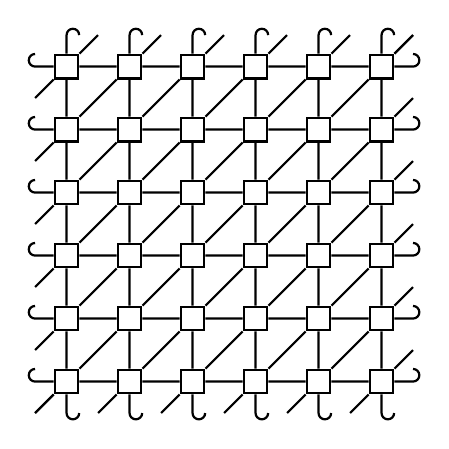
\begin{tikzpicture}[thick,scale=0.80]
			
			\def\width{6}
			\def\height{6}
			\pgfmathtruncatemacro{\widthh}{\width - 1}
			\pgfmathtruncatemacro{\heightt}{\height - 1}
			
			\def\lsize{0.1}
			\def\osize{0.5}
			
			\begin{scope}[minimum size=0.25cm,inner sep=0]
				\foreach \y in {1,...,\height}{
					\foreach \x in {1,...,\width}{
						\node (chip-\x-\y) at (\x,\y) [draw,fill=white,rectangle,minimum size=0.30cm,inner sep=0] {};
					}
				}
			\end{scope}
			
			% The obvious internal links
			\foreach \y in {1,...,\heightt}{
				\foreach \x in {1,...,\widthh}{
					\pgfmathtruncatemacro{\xx}{\x+1}
					\pgfmathtruncatemacro{\yy}{\y+1}
					\draw (chip-\x-\y) -- (chip-\xx-\yy);
					
					\pgfmathtruncatemacro{\xx}{\x+1}
					\pgfmathtruncatemacro{\yy}{\y+0}
					\draw (chip-\x-\y) -- (chip-\xx-\yy);
					
					\pgfmathtruncatemacro{\xx}{\x+0}
					\pgfmathtruncatemacro{\yy}{\y+1}
					\draw (chip-\x-\y) -- (chip-\xx-\yy);
				}
			}
			
			% The non-loop upper/right links
			\foreach \y in {1,...,\heightt}{
				\pgfmathtruncatemacro{\yy}{\y+1}
				\draw (chip-\width-\y) -- (chip-\width-\yy);
			}
			\foreach \x in {1,...,\widthh}{
				\pgfmathtruncatemacro{\xx}{\x+1}
				\draw (chip-\x-\height) -- (chip-\xx-\height);
			}
			
			% The looping left/right links
			\foreach \y in {1,...,\height}{
				\draw 
					(chip-\width-\y) -- ++(\osize,0) arc (-90:90:\lsize);
				\draw  (chip-1-\y) -- ++(-\osize,0) arc (90:-90:-\lsize);
			}
			
			% The looping up/down links
			\foreach \x in {1,...,\width}{
				\draw  (chip-\x-\height) -- ++(0,\osize) arc (180:0:\lsize);
				\draw  (chip-\x-1)       -- ++(0,-\osize) arc (-180:0:\lsize);
			}
			
			% The looping diagonal links
			\foreach \x in {1,...,\width}{
				\draw  (chip-\x-\height) -- ++(\osize,\osize);
				\draw  (chip-\x-1)       -- ++(-\osize,-\osize);
			}
			\foreach \y in {1,...,\height}{
				\draw  (chip-\width-\y) -- ++(\osize,\osize);
				\draw  (chip-1-\y)      -- ++(-\osize,-\osize);
			}
			
		\end{tikzpicture}
